\chapter{小世界复杂网络的混沌动力学}
\section{Duffing-WS型小世界网络基本模型}
Duffing 方程作为研究最为充分的混沌连续动力系统模型之一,具有丰富的非线性动力学行为 [15]。规范化的 Holmes型 Duffing 方程如下:
\begin{equation}
    \ddot{x}=-\gamma \dot{x}+a x-b x^{3}+A \sin (\Omega t)
\end{equation}
此方程具有三个平衡点:$S=(0,0),F_1=\left(\sqrt{\frac{a}{b}},0\right),F_2=\left(-\sqrt{\frac{a}{b}},0\right)$。
其中$F_1,F_2$是稳定的焦点,而$S$是不稳定的鞍点。当外加周期驱动力不存在(即$A=0$)时,受迫的Holmes型 Duffing方程(1)
退化为无摄动的Duffing方程,方程的解$x\left(t\right)$将以螺旋形式(衰减振荡)趋于两稳定焦点之一,并且初始条件决定着系统将最终趋于哪一焦点。
在其他参数固定的条件下,周期驱动力的幅值A从0开始逐渐增加到1时,方程的解会经历同宿轨道、分岔、混沌和大尺度周期等各个状态。

基于上述经典的Holmes型 Duffing 方程(3.1),本文提出如下具有N个节点的以WS小世界网络方式进行连接的Duffing复杂网,即Duffing- WS型小世界网络,其动力学方程为:
\begin{equation}
    \ddot{x}_{i}=-\gamma \dot{x}_{i}+a x_{i}-b x_{i}{ }^{3}+\varepsilon \sum_{j=1}^{N} a_{i j}\left(x_{j}-x_{i}\right)+A \sin (\Omega t), i=1,2, \ldots, N
\end{equation}
其中,$A\sin(\Omega t)$为周期驱动力,$x_i(t)$为第i个节点的输出, $i=1,2,\ldots,N$。 表示其它节点对第i个节点的耦合作用项, 称为耦合项,
$\left(a_{ij}\right)_{N\times N}$为网络的邻接矩阵,$\varepsilon$为网络耦合强度。这里我们采用Watts 和 Strogatz 提出的WS小世界网络作为拓扑网络结构[3]。
首先, N个节点连接形成一个规则的相邻网络,每个节点与它最近邻的K个节点相连,K称为重连度; 而后以概率p (称为重连概率)随机地重新连接网络中的每条边, 
即将边的一个端点保持不变, 而另一个端点取为随机选择的一个节点, 且规定任意两个不同的节点之间至多只能有一条边, 每一个节点都不能有边与自身相连。
对于WS小世界网络而言,当p = 0,模型为规则网;当p = 1时则为随机网;当0 < p < 1,则得到介于规则网与随机网之间的小世界网络。

通过引入Laplacian矩阵为$L=\left(l_{ij}\right)_{N\times N},l_{ij}=\begin{cases}
    -a_{ij},i\neq j \\ \sum_{j\neq i}a_{ij},i=j
\end{cases}$,则方程(3.2)可以改写为如下形式:
\begin{equation}
    \ddot{x}_{i}=-\gamma \dot{x}_{i}+a x_{i}-b x_{i}^{3}+A \sin (\Omega t)-\varepsilon\sum_{j=1}^{N} l_{i j} x_{j}
\end{equation}
由Laplacian矩阵的性质可知,L是一个实对称的弱对角占优矩阵,且对角元均非负,所以是半正定的。
\section{基本动力学特性研究}
\subsection{分岔图分析}
当驱动力幅度A值在(0,1)范围变化时,随着A值的变化,Duffing-WS小世界网络的各个粒子输出也将呈现小尺度周期运动、
倍周期分岔、混沌和大尺度周期运动等状态。这里,我们首先借助庞加莱截面给出Duffing-WS小世界网络的分岔图。
所谓分岔是指对于含参数的系统,当参数变动并经过某些临界值时,系统的定态性质(如平衡状态或者周期运动的数目和稳定性)
会发生突然的变化。分岔图则绘制了系统的庞加莱截面输出随参数的变化图,可用于比较微小参数扰动对系统指标的影响,
是系统稳定性的直观衡量,在本文中用来衡量混沌现象。
取庞加莱截面为$t=j T, T=2 \pi / \Omega$,在此截面上引入如下宏观变量$\sigma(j T)$来描述系统的集体行为:
\begin{equation}
    \sigma(j T)=\frac{1}{N} \sum_{i=1}^N x_i(j T)
\end{equation}
图(a)中给出了借助庞加莱截面单个 Duffing 方程的解随驱动力幅度 $A$ 变化的分岔图。图 (b) 给出了借助 $\sigma(j T)$, 
节点个数为 $N=100$ 的 Duffing-WS 型 小世界网络关于幅度 $A$ 的变化的分岔图。和图 1 中单个 Duffing 方程关于幅度 $A$ 
的分岔图对比可知, Duffing-WS 型小世界网络的分岔图事实上也历经了小尺度 周期运动、倍周期分岔、混沌和大尺度周期运动等状态,
 在大尺度周期状态之 后又进入了短暂的混沌状态, 因此其分岔图具有更为复杂的特性。
 \begin{figure}[!htbp]
    \centering
    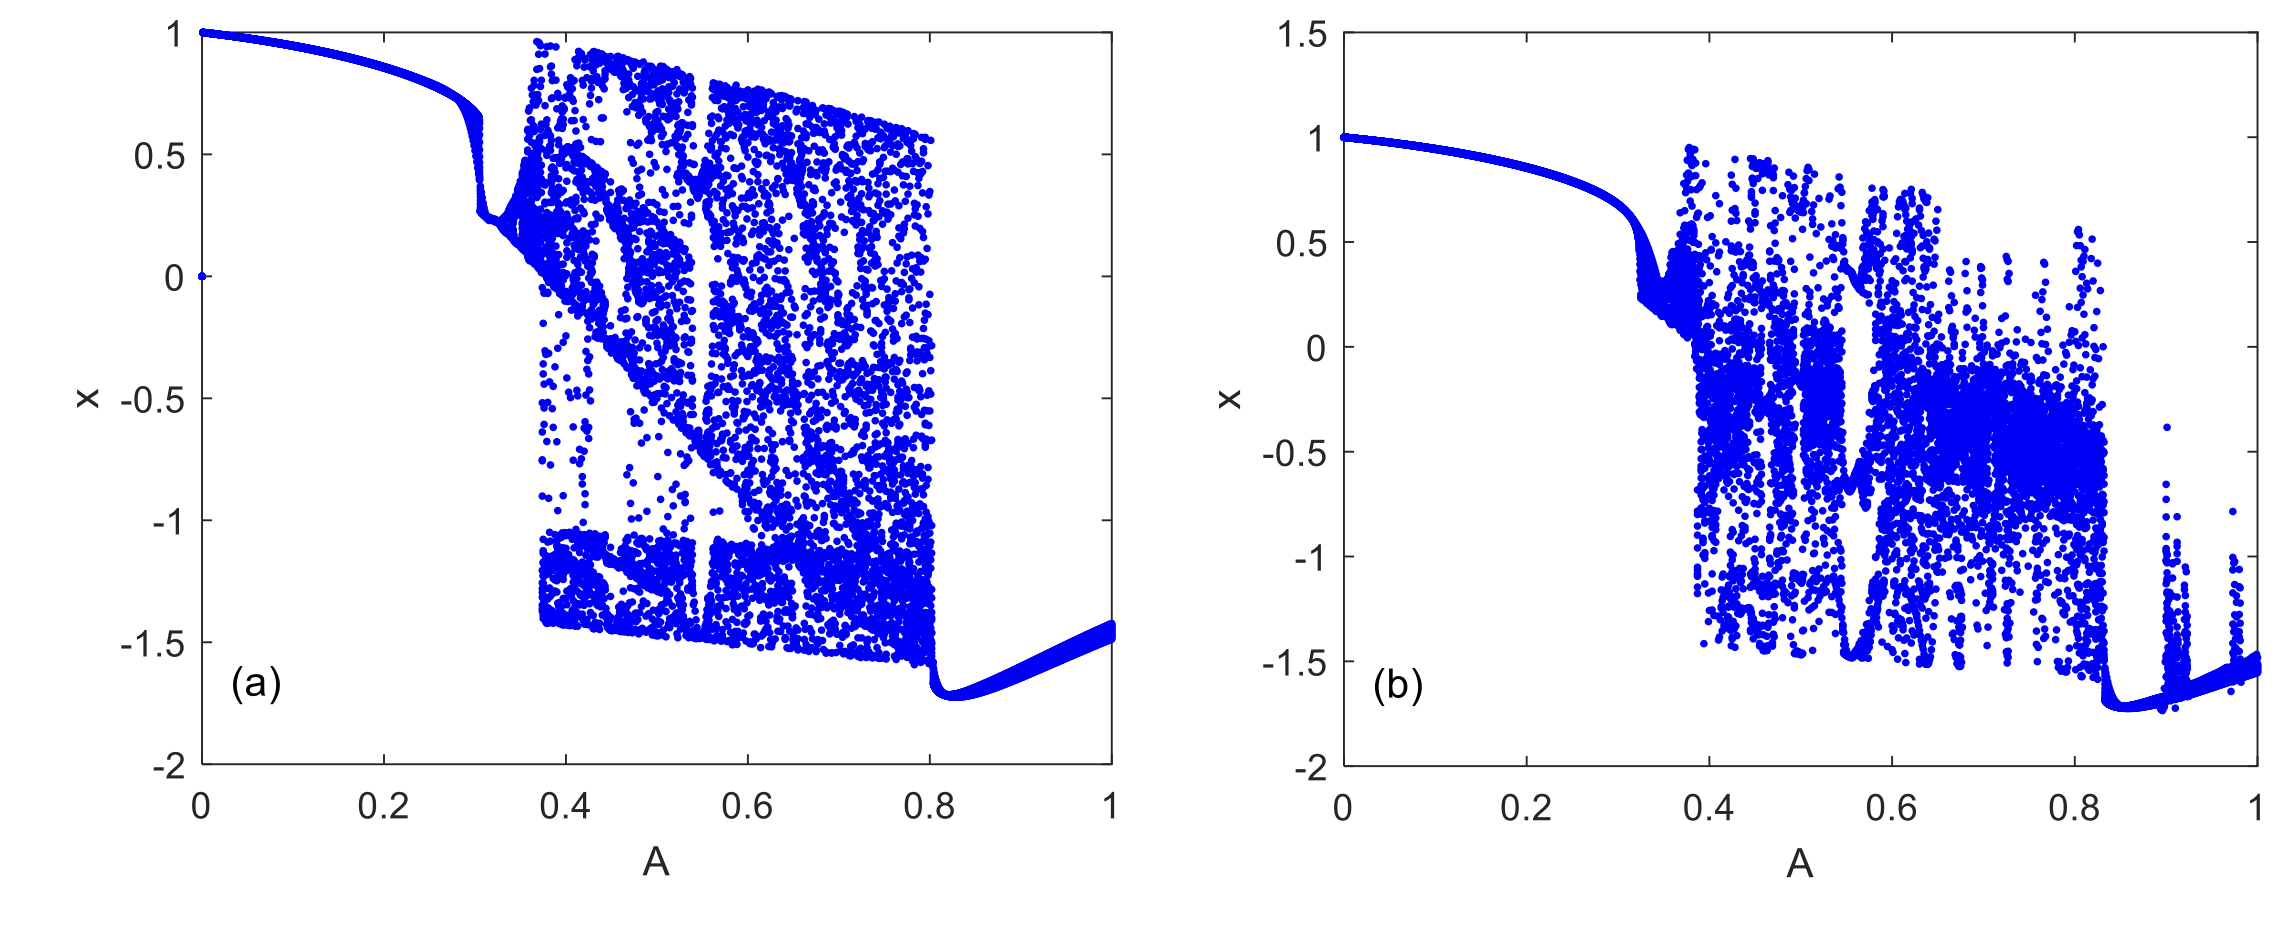
\includegraphics[width=0.8\textwidth]{31.png}
 \end{figure}
\subsection{李雅普诺夫指数分析}
 从3.1节可以看出,通过分岔图并不容易定量分析复杂系统的混沌行为,而对耦合系统混沌进行分析的另外一个指标为系统的最大Lyapunov指数
 (LE指数)。LE指数是衡量系统动力学特性的一个重要定量指标,表现了系统在相空间中相邻轨道间收缩或发散的平均指数率。
 对于系统是否存在动力学混沌,可以从最大LE指数是否大于零非常直观的判断出来: 一个正的LE指数,意味着在系统相空间中,
 无论初始两条轨线的间距多么小,其差别都会随着时间的演化而成指数率的增加以致达到无法预测,这就是混沌现象。
 这一节我们利用变分法推导 Duffing-WS 型小世界网络的最大 LE 指数表 达式, 利用最大 LE 指数来研究其混沌现象, 
 并分析小世界网络重连度 $K$, 重连 概率 $p$ 和耦合强度 $\varepsilon$ 等对复杂系统处于混沌运动状态参数范围的影响。
 通过令 $z_i=\Omega t,\left. z_i\right|_{t=0}=0$ 可将非自治方程变成如下的自治方程组:
 \begin{equation}
    \left\{\begin{array}{l}
    \dot{x}_i=y_i \\
    \dot{y}_i=-\gamma y_i+a x_i-b x_i^3+A \sin \left(z_i\right)-\varepsilon \sum_{j=1}^N l_{i j} x_j \\
    \dot{z}_i=\Omega
    \end{array}\right.
\end{equation}
假设 $s(t)$ 是单个 Duffing 方程(1)的解, 引入变分 $\delta_{x i}=x_i(t)-s(t), \delta_{y i}=y_i(t)-$ $\dot{s}(t)$,
可得到 Duffing-WS 小世界网络的变分方程为:
\begin{equation}
    \left\{\begin{array}{l}
    \dot{\delta}_{x i}=\delta_{y i} \\
    \dot{\delta}_{y i}=-\gamma \delta_{y i}+a \delta_{x i}-3 b x_i^2 \delta_{x i}+A \cos \left(z_i\right) \delta_{z i}-\varepsilon \sum_{j=1}^N l_{i j} \delta_{x j} \\
    \dot{\delta}_{z i}=0
    \end{array}\right.
\end{equation}
在不失去普遍性的情况下, 在上述变分方程中令集合 $\delta_{z i}=0$, 则变分方程可以简化为:
\begin{equation}
    \left\{\begin{array}{l}
    \dot{\delta}_{x i}=\delta_{y i} \\
    \dot{\delta}_{y i}=-\gamma \delta_{y i}+a \delta_{x i}-3 b x_i^2 \delta_{x i}-\varepsilon \sum_{j=1}^N l_{i j} \delta_{x j}
    \end{array}\right.
\end{equation}
则本文所提Duffing-WS型小世界网络的最大LE指数表达式为:
\begin{equation}
    \lambda_{\max }=\lim _{T \rightarrow \infty} \frac{\log \left(\sqrt{\sum_{i=1}^N\left|\delta_{x i}(T)\right|+\left|\delta_{y i}(T)\right|}\right)}{T}
\end{equation}
\subsection*{耦合强度$\varepsilon$对混沌的影响}
图(a)-(c)给出了不同的耦合强度 $\varepsilon$ 下平均最大 LE 指数随幅度 $A$ 变化的曲线, 重连概率均为 $p=0.5$ 。
在图(a)中 $K=2$, 当耦合强度 $\varepsilon$ 较小时 (如 $\varepsilon=0,0.2,0.4)$, 随着 $\varepsilon$ 的增大,
LE 指数大于 0 的混沌区域扩大; 当耦合强度 $\varepsilon$ 较大时 (如 $\varepsilon=$ $0.6,0.8,1,2)$, 
随着 $\varepsilon$ 的增加, LE 指数大于 0 的混沌区域则逐渐收缩, 混沌受到抑制。在这种情况下, 
由于重连度非常小节点之间的连接程度不够, 小的耦合强 度的增强反而增强系统的混沌运动; 而只有耦合强度大到一定程度, 
更大的耦合强度使得系统协同性增强, 才能抑制系统的混沌运动。\par
在图(b)中 $K=20$, 可以看到, 当 $\varepsilon=0$ 时, 小世界网络退化成独立的 $N$ 个 Duffing系统, 此时混沌区域最大, 
而当 $\varepsilon>0$ 时, 小世界网络各个节点之间存在 耦合作用, 网络的混沌区域收缩; 而此时由于重连度 $K$ 值较大, 平均 LE 指数随
幅度 $A$ 变化的曲线在不同的耦合强度 $\varepsilon$ 下基本一致, 也就是说此时小世界网络的混沌运动区域对耦合强度 
$\varepsilon$ 具有鲁棒性。同样, 在图(c)中 $K=48$, 可以看到, 随着 $\varepsilon$ 增加, 混沌区域的变化同样不明显。
综上可以看到, 和传统的规则网络不同, 本文所提 Duffing-WS 型小世界网络的耦合强度 $\varepsilon$ 
对混沌区域的影响并不是线性的, 当重连度 $K$ 较小时, 随着耦合强度的增加混沌区域呈现出先扩大后缩小的变化, 
$K$ 较大时 $\varepsilon$ 的增强对混沌区域影响不明显。
\begin{figure}[!htbp]
    \centering
    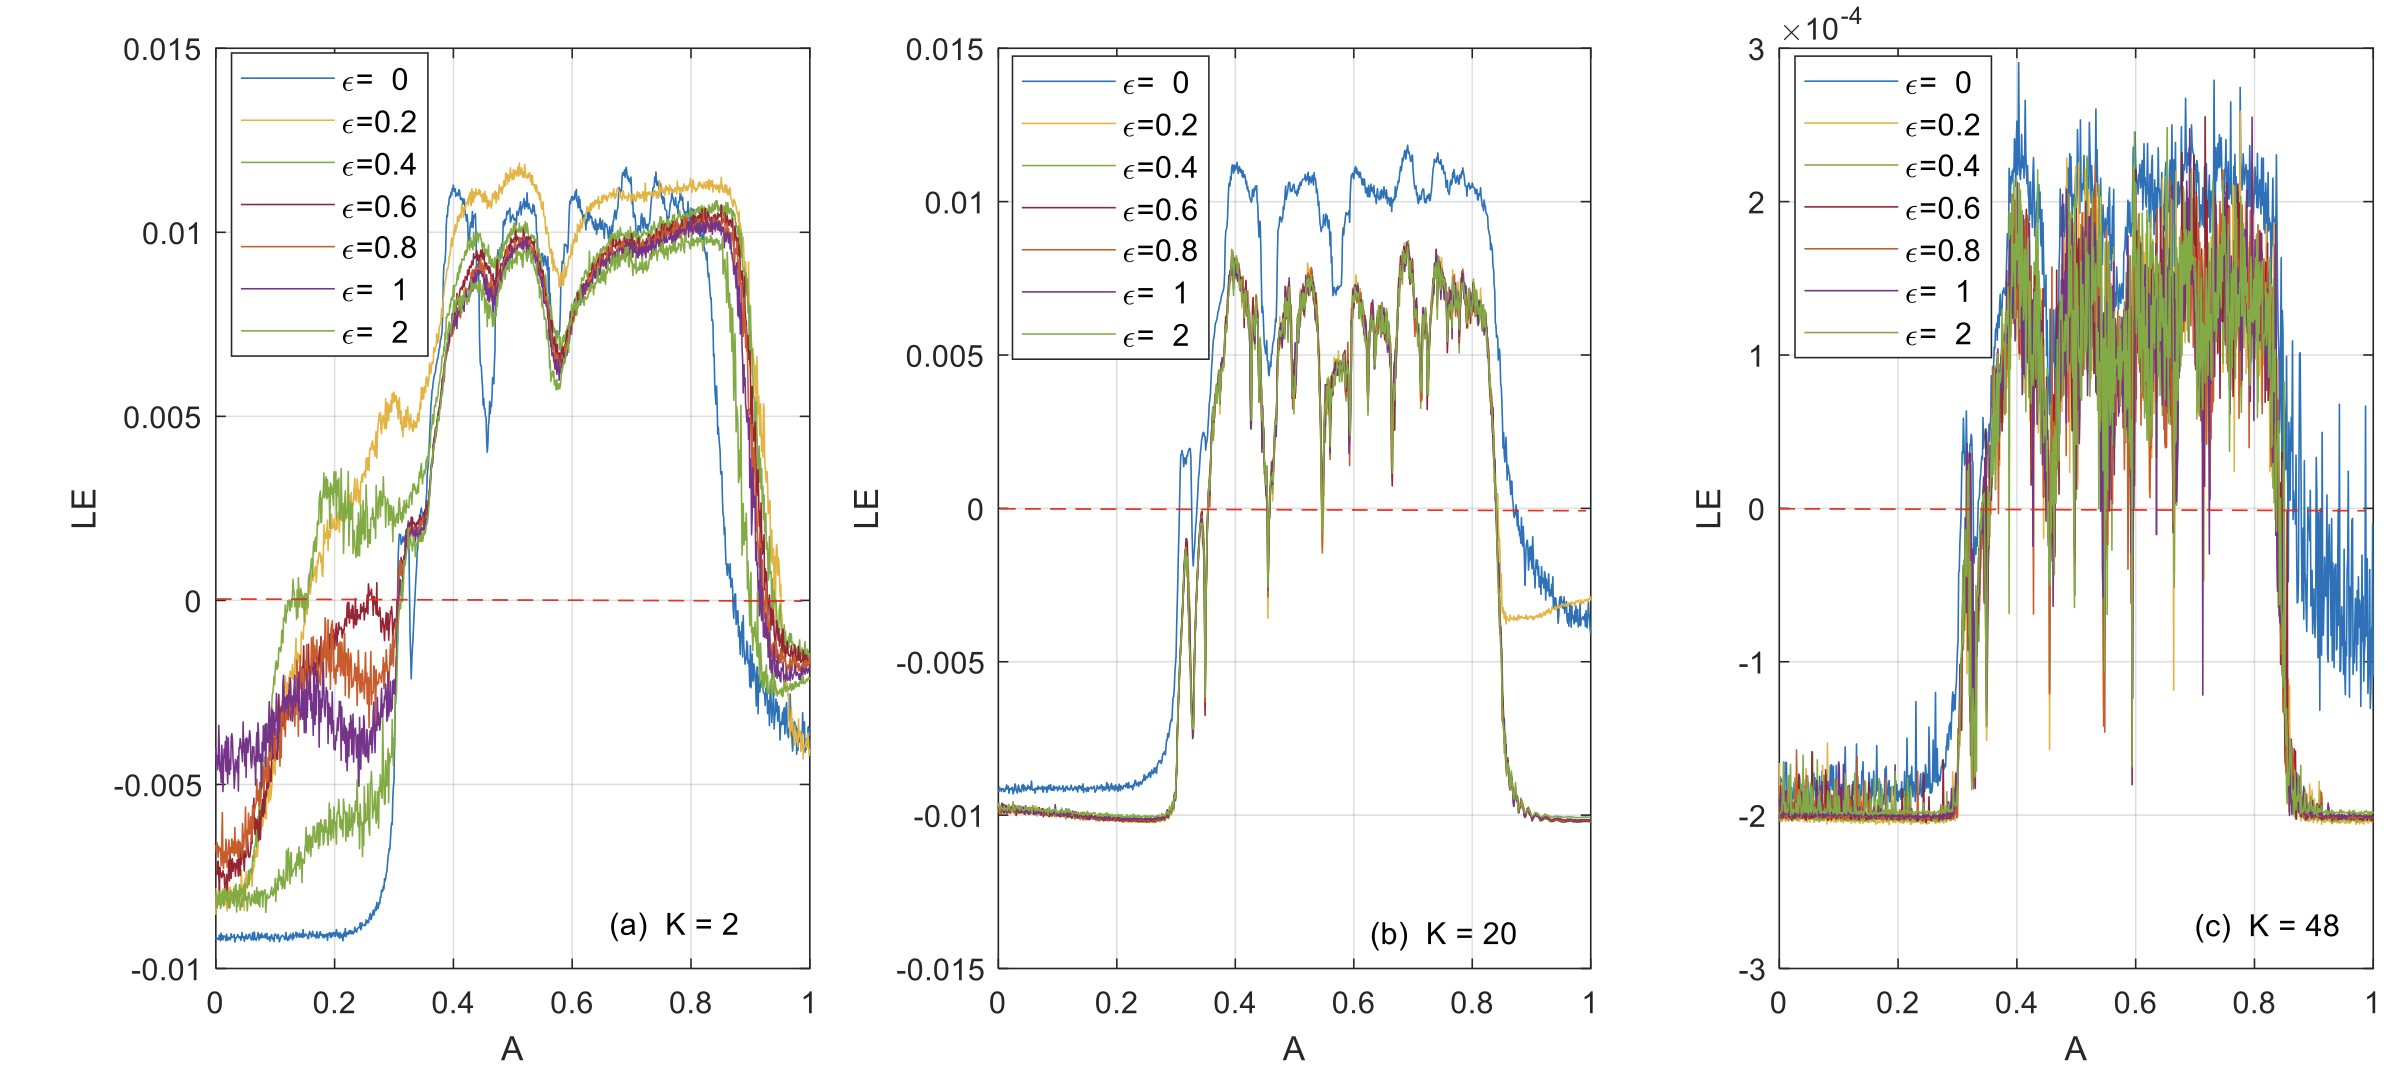
\includegraphics[width=\textwidth]{32.png}
\end{figure}
\subsection*{重连度$K$对混沌的影响}
图(a)-(c)给出了不同的重连度 $K$ 下平均 LE 指数随幅度 $A$ 变化的曲线, 耦合 强度均为 $\varepsilon=0.5$ 。
可以看出, 在图(a)中 $p=0$, 耦合网络为规则的最近邻耦合 网络, 当重连度 $K$ 较小时 $(K=2,4,6,8,10)$, 
随着重连度 $K$ 的增加, LE 指数大于 0 的混沌区域先扩大再收缩, 当 $K=4$ 时混沌区域达到最大; 随后,
随着重连度 $K$ 增加到一定程度以后 $(K=20,30,40,48)$, 混沌区域随着 $K$ 值的增加而有略微地缩小, 
但总体上差异不大。这说明对于规则网络, 只有足够大的重连度才会抑制 系统混沌, 较小的重连度反而增加系统的混沌运动。\par
在图(b)中 $p=0.5$, 此时网络为标准的小世界模型。 $K=2$ 与$K$ 值 LE 曲线 有显著不同, 所对应的混沌区域最大,
LE 指数在各个振幅处的值都最高, 可见 重连度 $K$ 较低时更容易产生较大的混沌范围。 $K=4,6$ 比起 $K=2$ 的 LE 曲线, 其
大于 0 的区域明显缩小, 即重连度的增加明显抑制了网络混沌运动; 随着 $K$ 值进 一步增加, 系统 LE 曲线几乎没有变化, 
这是因为当重连度足够高时, 系统各节 点输出间差异很小, 混沌区域几乎一致。\par
在图 (c)中 $p=1$, 此时网络为完全的随机网络。可以看出, $K$ 足够大时 LE 曲线的一致性会被打破,
重连度对混沌区域的控制不再呈现明显的规律。当 $K=2$ 时混沌区域反而最小, 而中间大小的重连度 $(K=4,6,8,10)$ 混沌区域却最大。
同时, 对比完全规则网络 $(p=0)$ 与小世界网络 $(p=0.5)$, 完全随机网络的混 沌区域更大且 LE 指数更低。
\begin{figure}[!htbp]
    \centering
    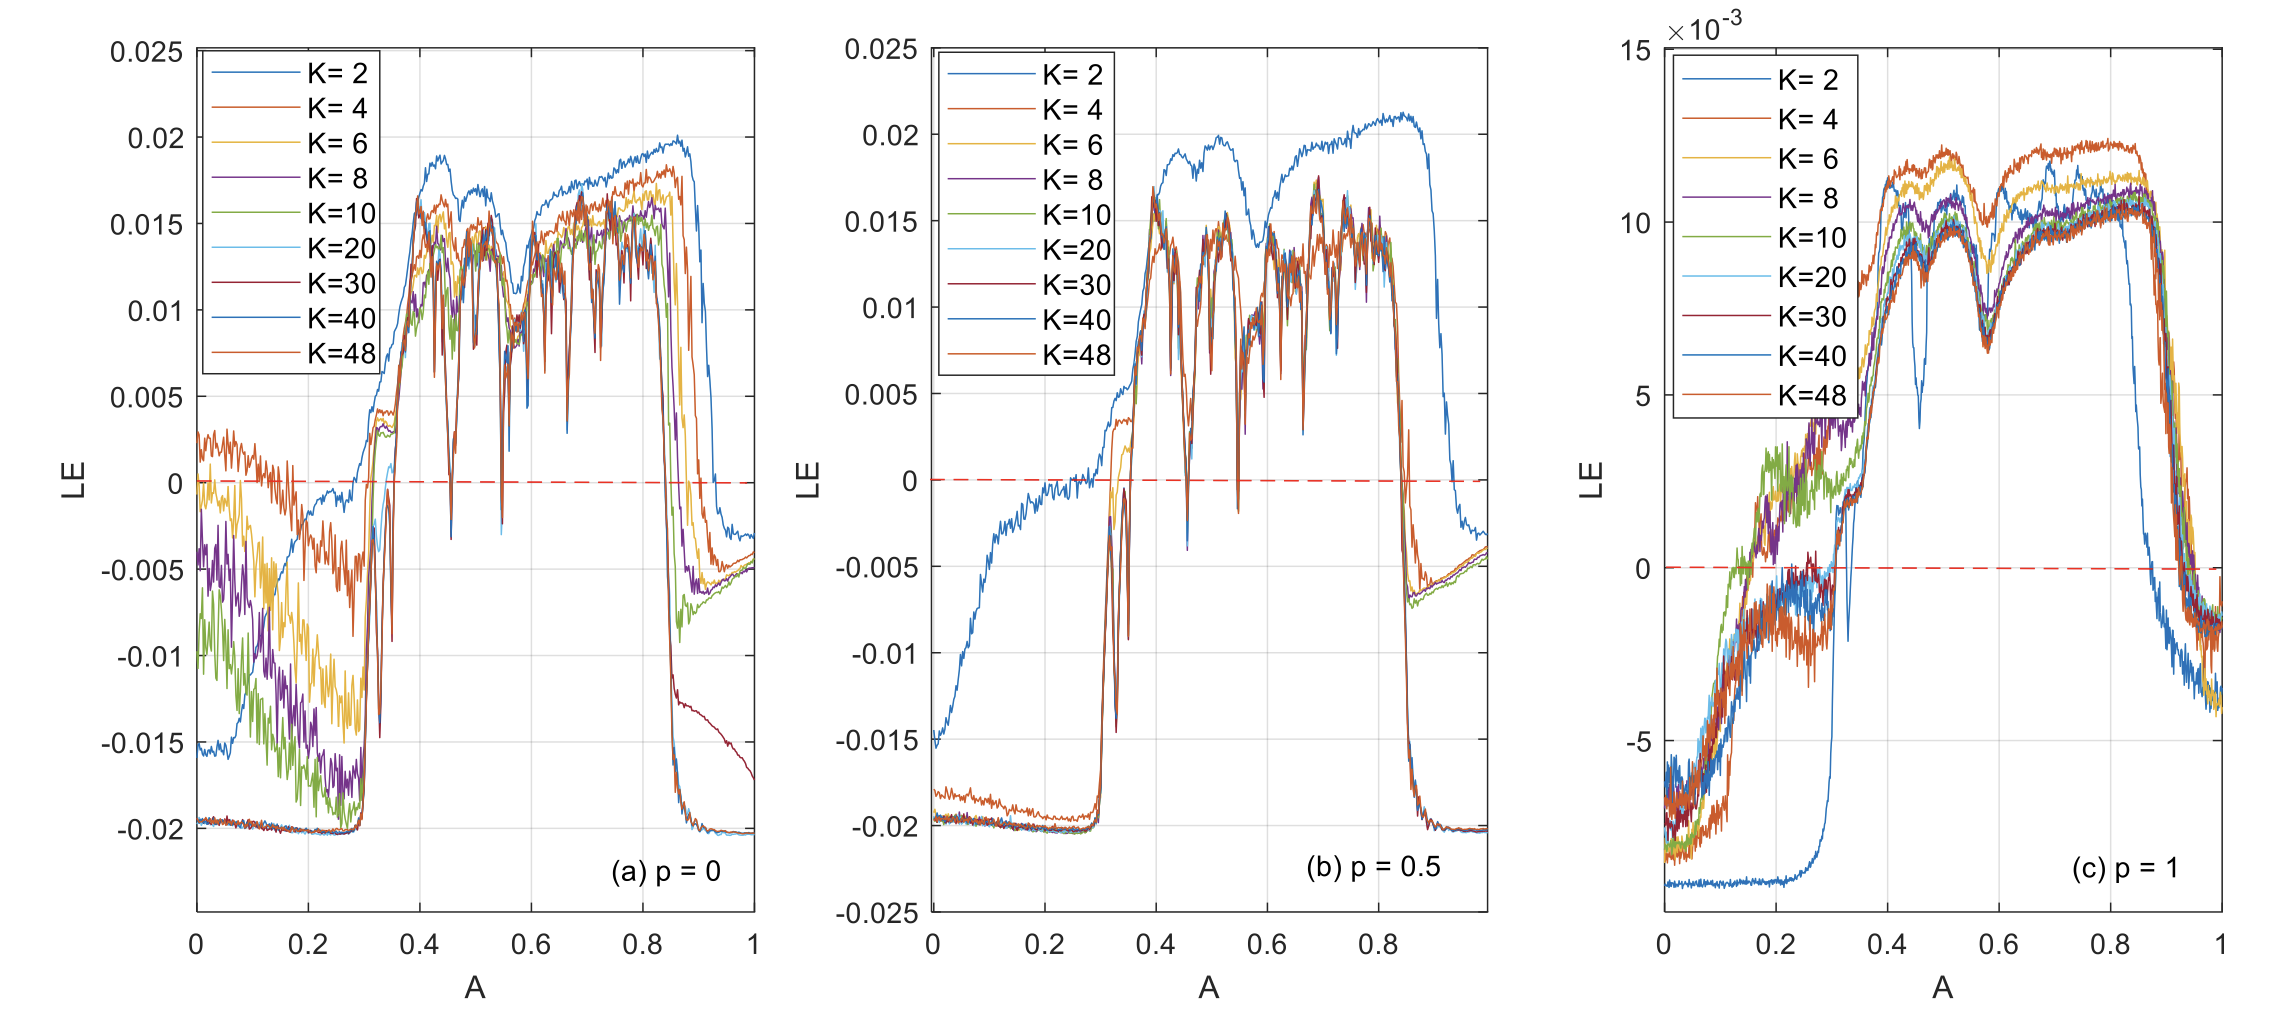
\includegraphics[width=\textwidth]{33.png}
\end{figure}
\subsection*{重连概率$p$对混沌的影响}
图(a)-(c)给出了不同的重连概率 $p$ 下平均LE指数随幅度 $A$ 变化的曲线, 耦 合强度均为 $\varepsilon=0.5$ 。
在图 (a)中 $K=2$, 在图(b)中 $K=20$, 可以看出, 不同重 连概率 $p$ 对混沌区域的影响不明显, 
差异主要体现在 LE 指数的高低上, 重连概 率 $p$ 越大, LE 指数值越小。在图中 $K=48$, 在这种情形下混沌区域明显后
移。总的来说,此时小世界网络的混沌区域对重连概率$p$具有鲁棒性。
\begin{figure}[!htbp]
    \centering
    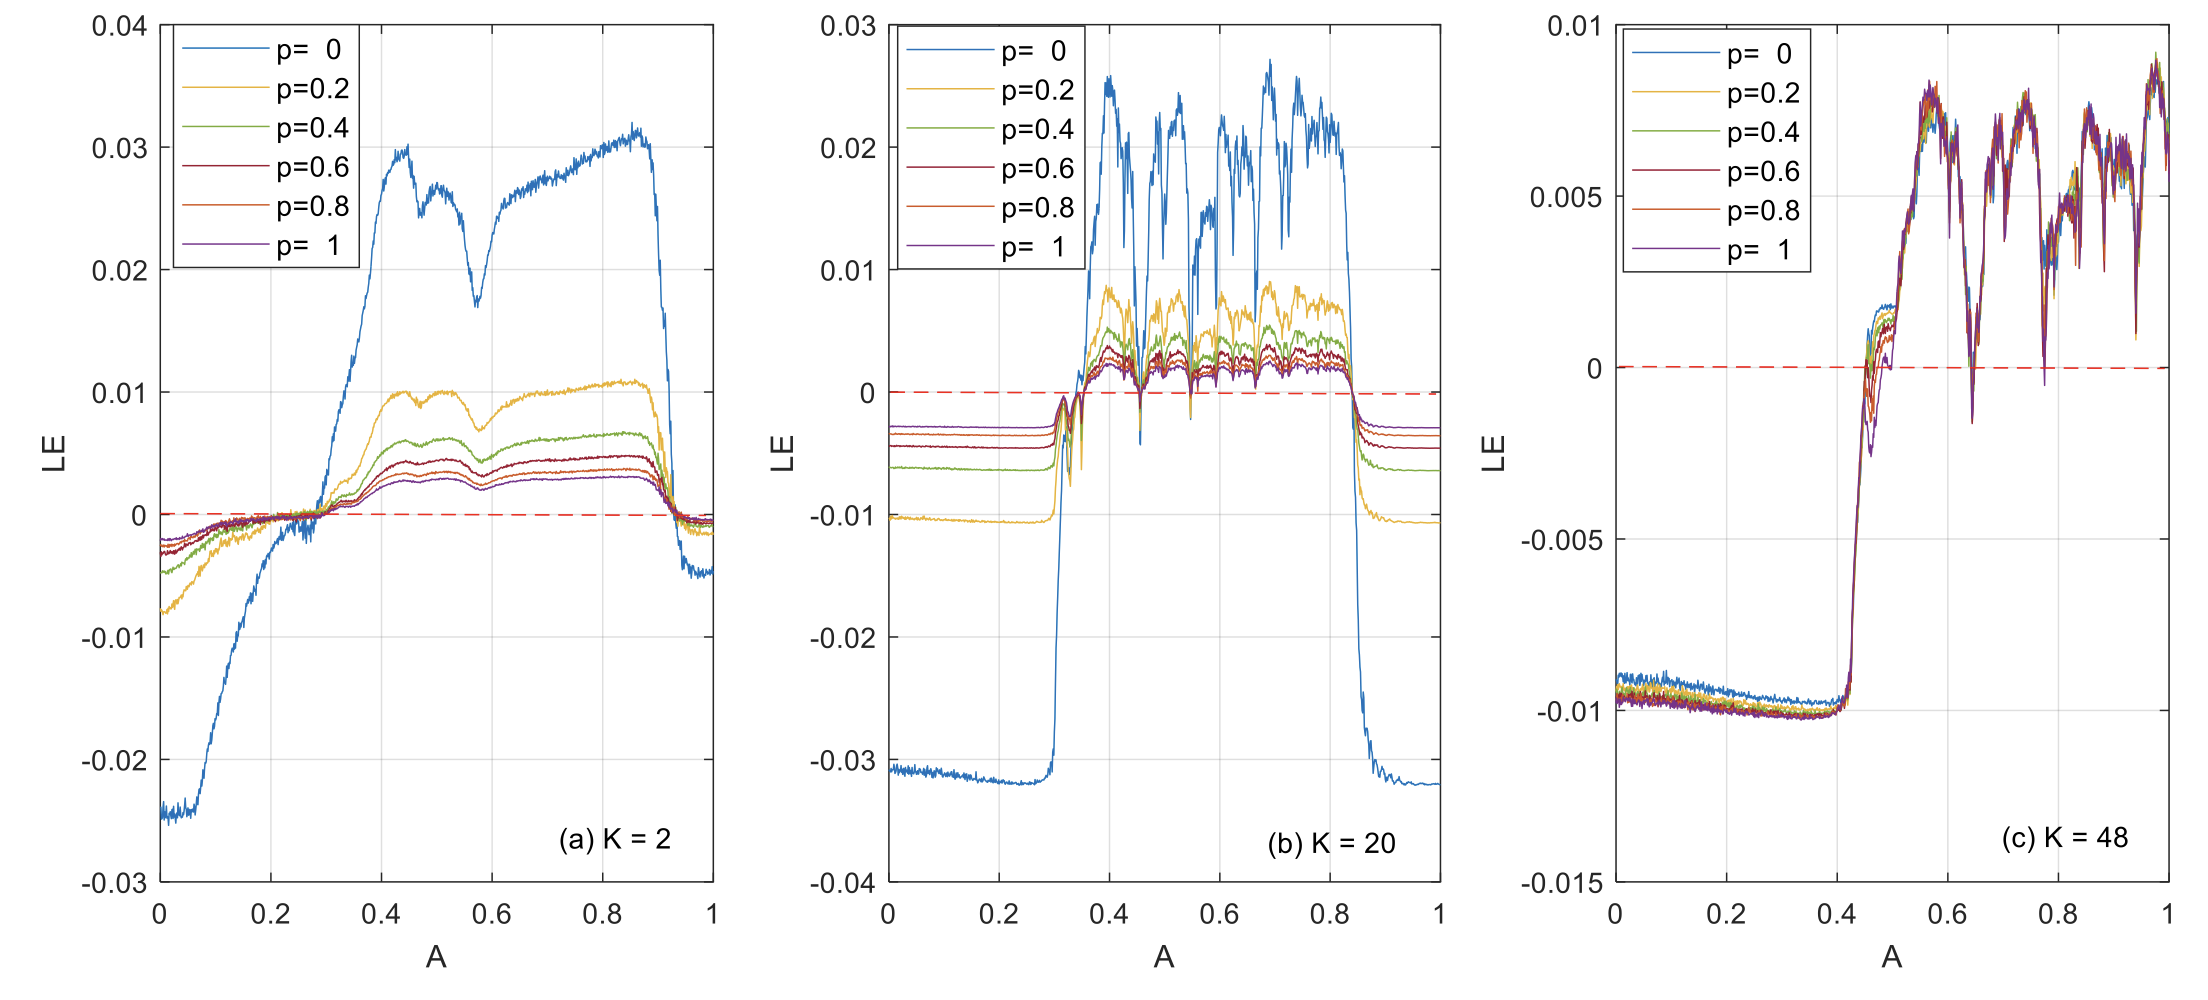
\includegraphics[width=\textwidth]{34.png}
\end{figure}
\subsection{同步性分析}
这一节中,我们给出Duffing-WS小世界网络的同步性分析。大量耦合粒子
的同步化问题最早由1998年给出的基于变分方程的主稳定函数方法而得到妥善地解决。\par
通过令 $z_i=\Omega t,\left.z_i\right|_{t=0}=0$ 可将非自治方程(3.3)变成自治方程组:
\begin{equation}
    \left\{\begin{array}{l}
    \dot{x}_i=y_i \\
    \dot{y}_i=-\gamma y_i+a x_i-b x_i^3+A \sin \left(z_i\right)-c \sum_{j=1}^N l_{i j} x_j \\
    \dot{z}_i=\Omega
    \end{array}\right.
\end{equation}
假设 $s(t)$ 是单个 Duffing 方程的解, 引入变分 $\delta_{x i}=x_i(t)-s(t), \delta_{y i}=y_i(t)-\dot{s}(t)$,
可得到Duffing-WS小世界网络的变分方程为:
\begin{equation}
    \left\{\begin{array}{l}
    \dot{\delta}_{x i}=\delta_{y i} \\
    \dot{\delta}_{y i}=-\gamma \delta_{y i}+a \delta_{x i}-3 b x_i^2 \delta_{x i}+A \cos \left(z_i\right) \delta_{z i}-c \sum_{j=1}^N l_{i j} \delta_{x j} \\
    \dot{\delta}_{z i}=0
    \end{array}\right.
\end{equation}
令 $\boldsymbol{\delta}_{:}=\left[\delta_2, \delta_2, \delta_{-}\right]^T$, Duffing-WS 小世界网络的变分方程可以简化为如下的矢量形式:
\begin{equation}
    \dot{\boldsymbol{\delta}}_i=D f(\mathbf{S}) \boldsymbol{\delta}_i-c \sum_{j=1}^N l_{i j} H \boldsymbol{\delta}_j, i=1,2, \ldots, N
\end{equation}
其中 $f(\mathbf{X})=\left[\begin{array}{c}y \\ -\gamma y+a x-b x^3+A \sin (z) \\ \Omega\end{array}\right]$ 为孤立节点动力学函数, 节点内连矩阵为
$H=\left[\begin{array}{lll}
0 & 0 & 0 \\
1 & 0 & 0 \\
0 & 0 & 0
\end{array}\right] $。
令同步流形为 $\mathbf{S}(t)=(s(t), \dot{s}(t), \Omega t)^T$, 即孤立节点动力学方程 $\dot{\mathbf{S}}(t)=f(\mathbf{S})$ 的解。
$D f(\mathbf{S})$ 则为单节点动力学函数在同步流形 $\mathbf{S}(t)=(s(t), \dot{s}(t), \Omega t)^T$ 处的雅可比矩阵, 有
\begin{equation}
    D f(\mathbf{S})=\left[\begin{array}{ccc}
    0 & 1 & 0 \\
    a-3 b s^2(t) & -\gamma & A \cos (\Omega t) \\
    0 & 0 & 0
    \end{array}\right]
\end{equation}
令 $\boldsymbol{\delta}=\left(\boldsymbol{\delta}_1, \ldots, \boldsymbol{\delta}_N\right)$, 则(3.11)式可以改写为
\begin{equation}
    \dot{\boldsymbol{\delta}}=D f(\mathbf{S}) \boldsymbol{\delta}-c H \boldsymbol{\delta} L^T
\end{equation}
不妨 假设 Laplacian矩阵可对角化 (即为无向图情况)), $L^T=P \Lambda P^{-1}, \Lambda=\operatorname{diag}\left(\lambda_1, \ldots, \lambda_N\right)$, 
令 $\boldsymbol{\eta}=\boldsymbol{\delta} P$, 则方程组又等价于如下的方程组:
\begin{equation}
    \begin{gathered}
    \dot{\boldsymbol{\eta}}_1=D f(\mathbf{S}) \boldsymbol{\eta}_1, k=1,2, \ldots, N \\
    \dot{\boldsymbol{\eta}}_k=\left[D f(\mathbf{S})-c \lambda_k H\right] \boldsymbol{\eta}_k, k=2, \ldots, N
    \end{gathered}
\end{equation}
第一式对应于与同步流形平行方向的扰动,为保证同步流形的稳定性,需要第二式描述的$N-1$个子系统是渐近稳定的。注意到除非$s(t)$是平衡点,
否则第二式中的每个子系统都是时变系统,判断同步流形稳定的一个常用判据是要求主稳定方程的所有Lyapunov指数全为负值。
所对应的主稳定方程可以写为:
\begin{equation}
    \dot{\boldsymbol{y}}=\boldsymbol{M}(\alpha)\boldsymbol{y}
\end{equation}
其中 $\boldsymbol{M}(\alpha)=\left[\begin{array}{ccc}0 & 1 & 0 \\ a-3 b s^2(t)-\alpha & -\gamma & A \cos (\Omega t) 
\\ 0 & 0 & 0\end{array}\right], \alpha=c \lambda_k$, 其最大李亚普洛夫指数 假设为 $L E(\alpha)$ 。
将主稳定方程和单个节点的方程联立,得到
\begin{equation}
    \left\{\begin{array}{l}
    \dot{s}_1=s_2 \\
    \dot{s}_2=-\gamma s_2+a s_1-b s_1^3+A \sin (\Omega t) \\
    \dot{y}_1=y_2 \\
    \dot{y}_2=\left(a-3 b s_1^2-\alpha\right) y_1-\gamma y_2+A \sin (\Omega t) y_3 \\
    \dot{y}_3=0
    \end{array}\right.
\end{equation}
则其最大 Lyapunov 指数为 $L E(\alpha)=\lim _{T \rightarrow+\infty} 
\frac{\ln \left(\left|y_1(T)\right|+\left|y_2(T)\right|\right)}{T}$。
下面的图绘制了当周期驱动幅度A在[0,1]范围内,
在平面Lyapunov指数的相图,其中黑色区域为最大Lyapunov指数非负即不同步的区域(按照不同初始值取了50次平均)。\par
\begin{figure}[!htbp]
    \centering
    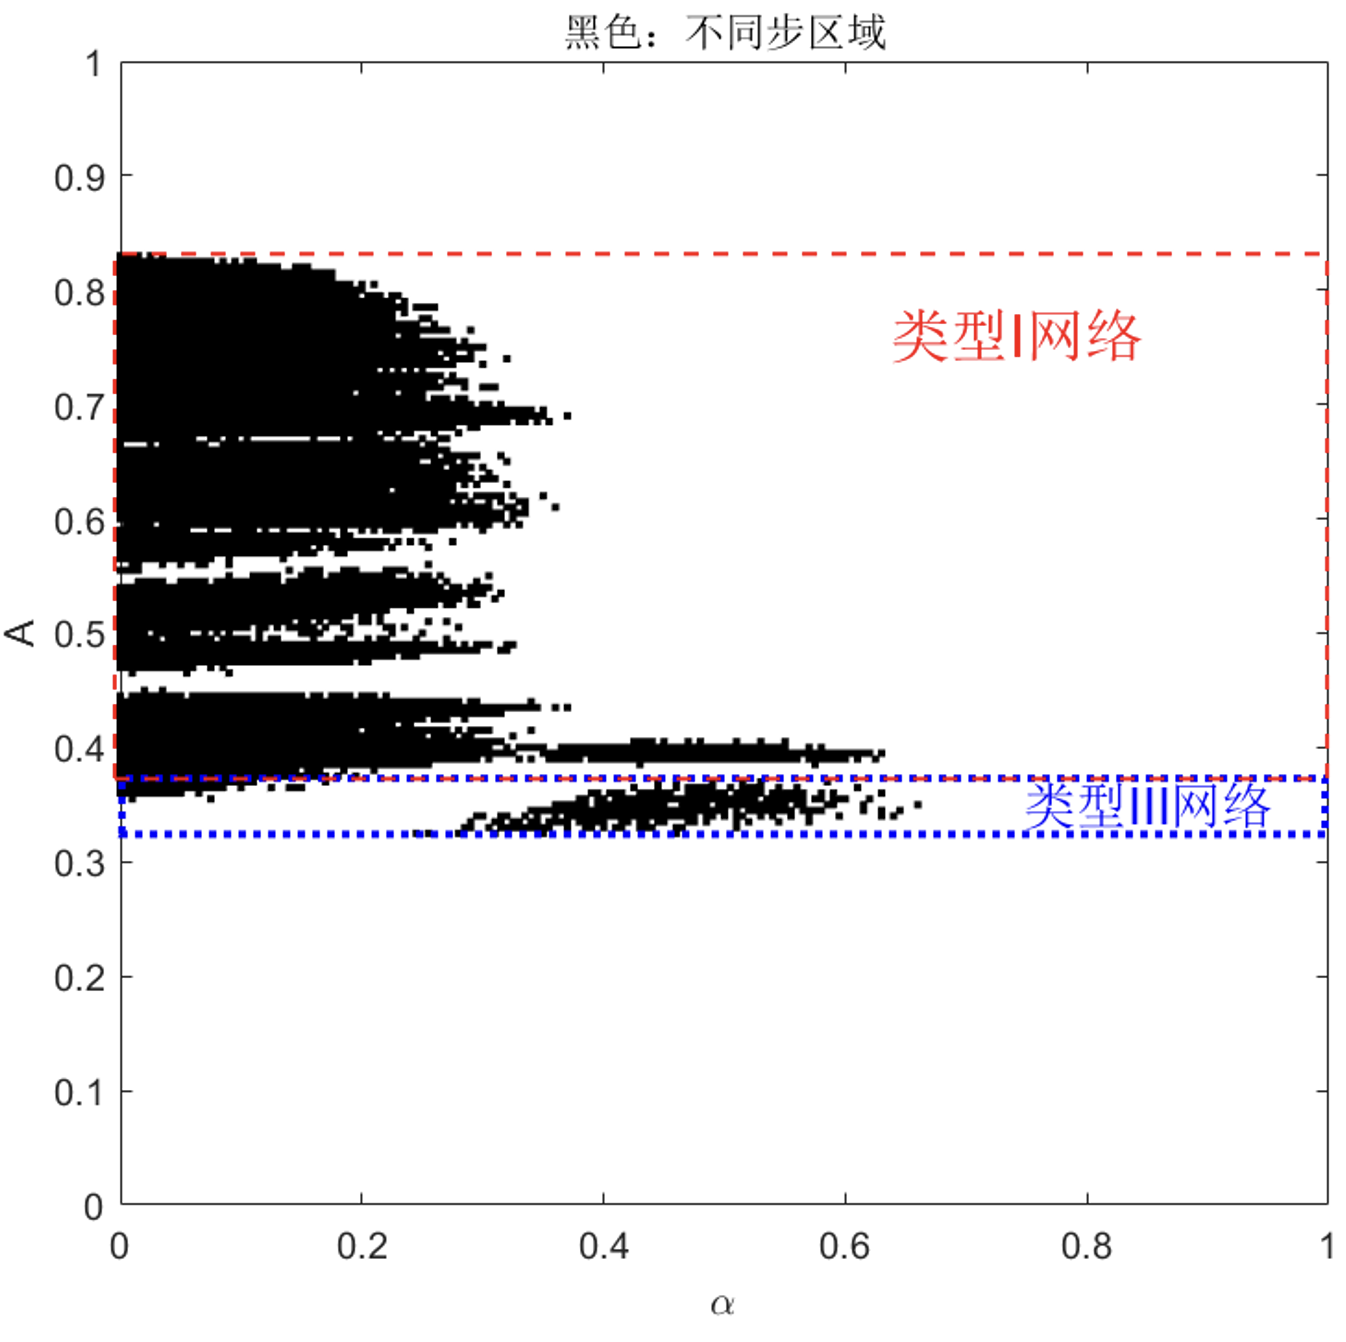
\includegraphics[width=0.8\textwidth]{tb1.png}
\end{figure}
当 $A \in[0,0.32] \cup[0.83,1]$ 时, 最大 $\mathrm{LE}$ 指数全为负数, 即为同步化区域为全区 域 $S R=(0,+\infty)$,
这时候的系统总是可以达到完全同步 (和耦合网络结构小世界特性无关);\par
当 $A \in[0.33,0.37]$ 时, 网络属于类型 III 的网络, 同步化区域为不连通的多区 域 $S R=\left(0, \alpha_1\right) \cup\left(\alpha_2,+\infty\right)$,
这时候系统要达到完全同步, 必须满足 $c \lambda_k \in S R, k=2,3, \ldots, N$, 
而要同时调整耦合强度和所有特征值全部落入不连通的同步化区域 SR 此时, 
如果满足 $c \lambda_2>\alpha_2$, 则 $\alpha_2<c \lambda_2 \leq \ldots \leq c \lambda_N$ 时, 
都有 $L E(\alpha)<0$, 同步流形总是稳定的, 系统总能同步。在这种情况下, Laplacian 矩阵的第二大特征值 
$\lambda_2$ 的大小可以作为衡量网络同步化能力的指标, $\lambda_2$ 越 大则系统越容易达到同步, 也就是系统的同步化能力越强。
如果 $\alpha_1<c \lambda_2<\alpha_2$, 则同步流形不稳定, 系统不能同步。如果 $c \lambda_2<\alpha_1$, 
则要求 $c \lambda_N<\alpha_1\left(\lambda_N / \lambda_2<c\right)$ 或者 $\alpha_2<c \lambda_3$, 则同步流形稳定, 
此时系统同步相对于前 面两种情况更不容易实现。\par
当 $A \in[0.38,0.82]$ 时, 网络属于类型 $\mathrm{I}$ 的网络, 同步化区域为无界区域 $S R=\left(\alpha_3,+\infty\right)$, 
即当 $\alpha_3<c \lambda_2 \leq \ldots \leq c \lambda_N$ 时, 都有 $L E(\alpha)<0$, 即 $c \lambda_2>\alpha_3$, 
同步流形总是稳定的, 系统总能同步。在这种情况下, Laplacian 矩阵的第二大 特征值 $\lambda_2$ 的大小可以作为衡量网络同步化能力的指标。\par
综上可知, 对于不同的 A 值, 当 Laplacian 矩阵的第二大特征值 $\lambda_2$ 和耦合系数的乘积 $c \lambda_2$ 充分大时, 
系统总能实现同步; 给定耦合系数 $\mathrm{c}$, Laplacian 矩阵 的第二大特征值 $\lambda_2$ 决定了系统的同步能力, 
当 $\lambda_2$ 的值较小时, 系统则很有可能 不能同步。但是当增加耦合系数 $\mathrm{c}$ 大于某个值时, 对于系统也总能实现同步。
下图给出了粒子个数为 $\mathrm{N}=20,100,1000$ 时, Duffing-WS 小世界网络 Laplacian 矩阵的第二大特征值 $\lambda_2$ 和
最大特征值 $\lambda_N$ 在不同的 $\mathrm{K}$ 值下随重连概率 $\mathrm{p}$
变化的曲线(平均 100 次), 可以看到当连接度较小 $(\mathrm{K}=1)$ 时, 第二大特征值 $\lambda_2$ 随着重连概率增加先减小后增加, 
说明此时较小或较大的重连概率均有利于增加系 统同步; 随着连接度增加(左图, $K=2,3,4,5,6$ ), 第二大特征值 $\lambda_2$ 
随着重连概率增加先增加后减小, 说明此时适当大小的重连概率有利于增加系统的同步; 当连接 度继续增加而接近 $\mathrm{N} / 2$ 时, 
第二大特征值 $\lambda_2$ 随着重连概率增加而减小, 说明较小 的重连概率有利于增加系统的同步。\par
\begin{figure}[!htbp]
    \centering
    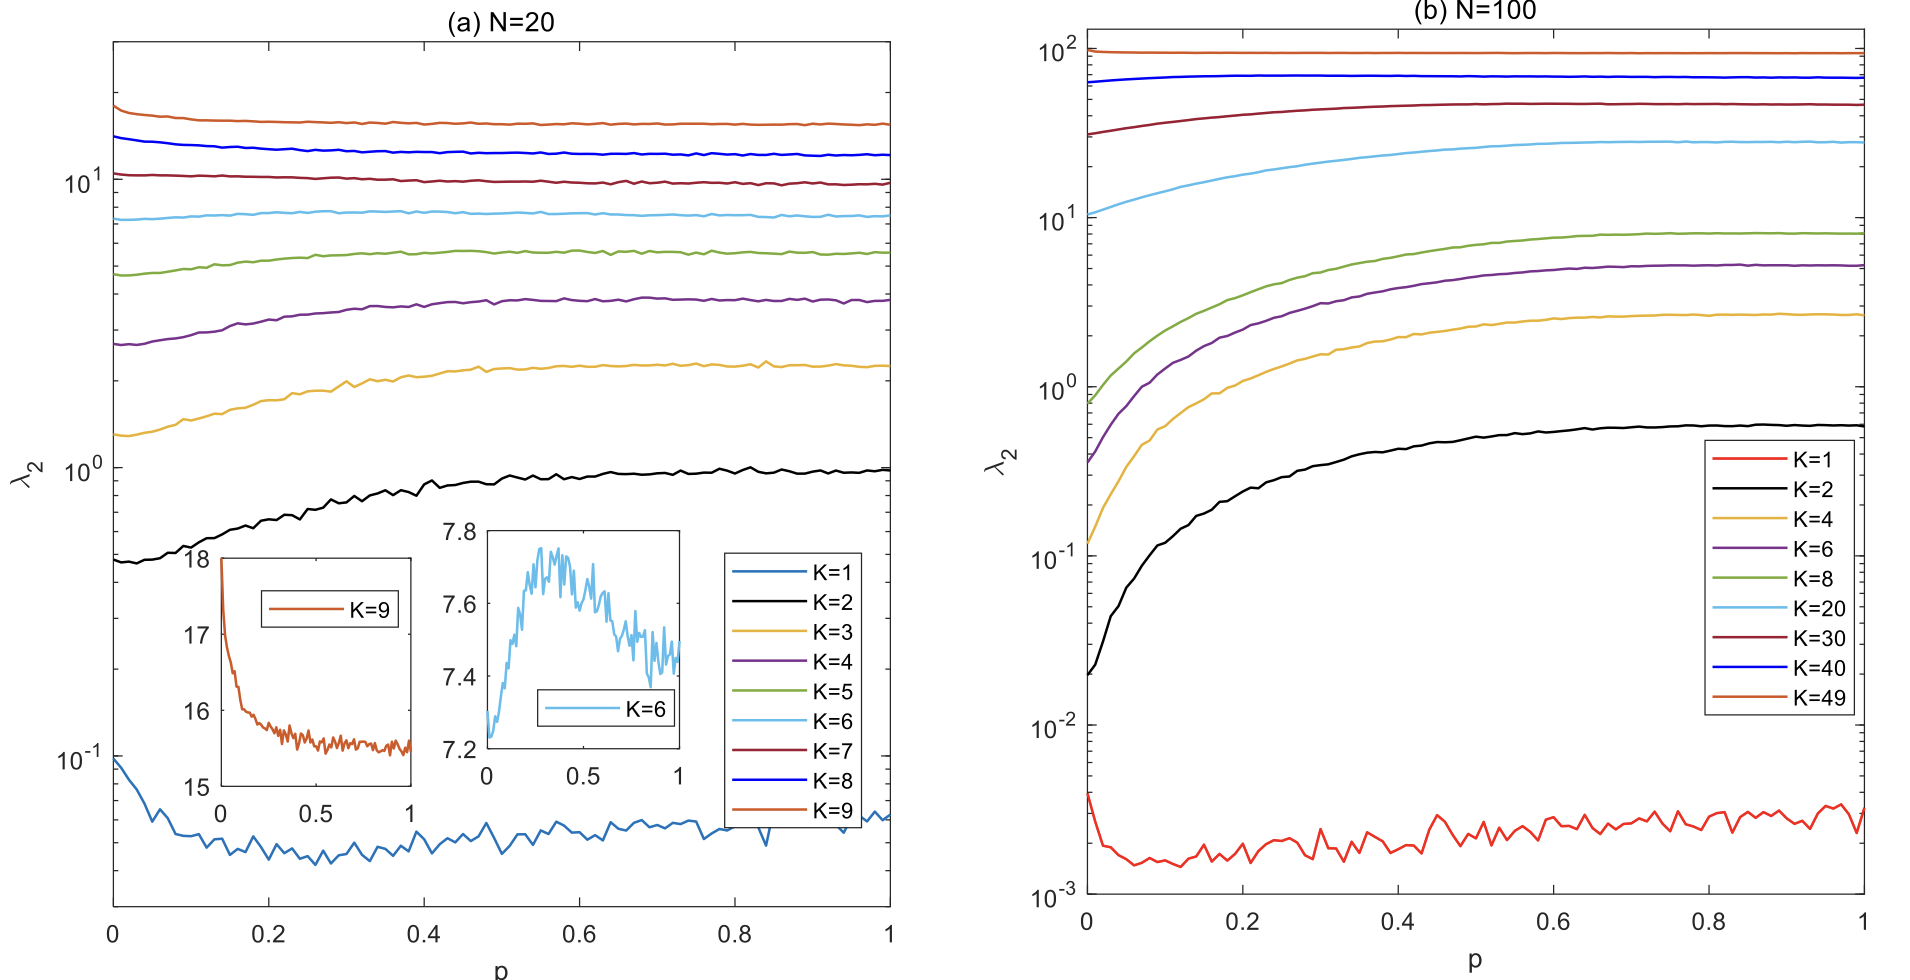
\includegraphics[width=\textwidth]{tb2.png}
\end{figure}
下面是N=1000的结果。\par
\begin{figure}[!htbp]
    \centering
    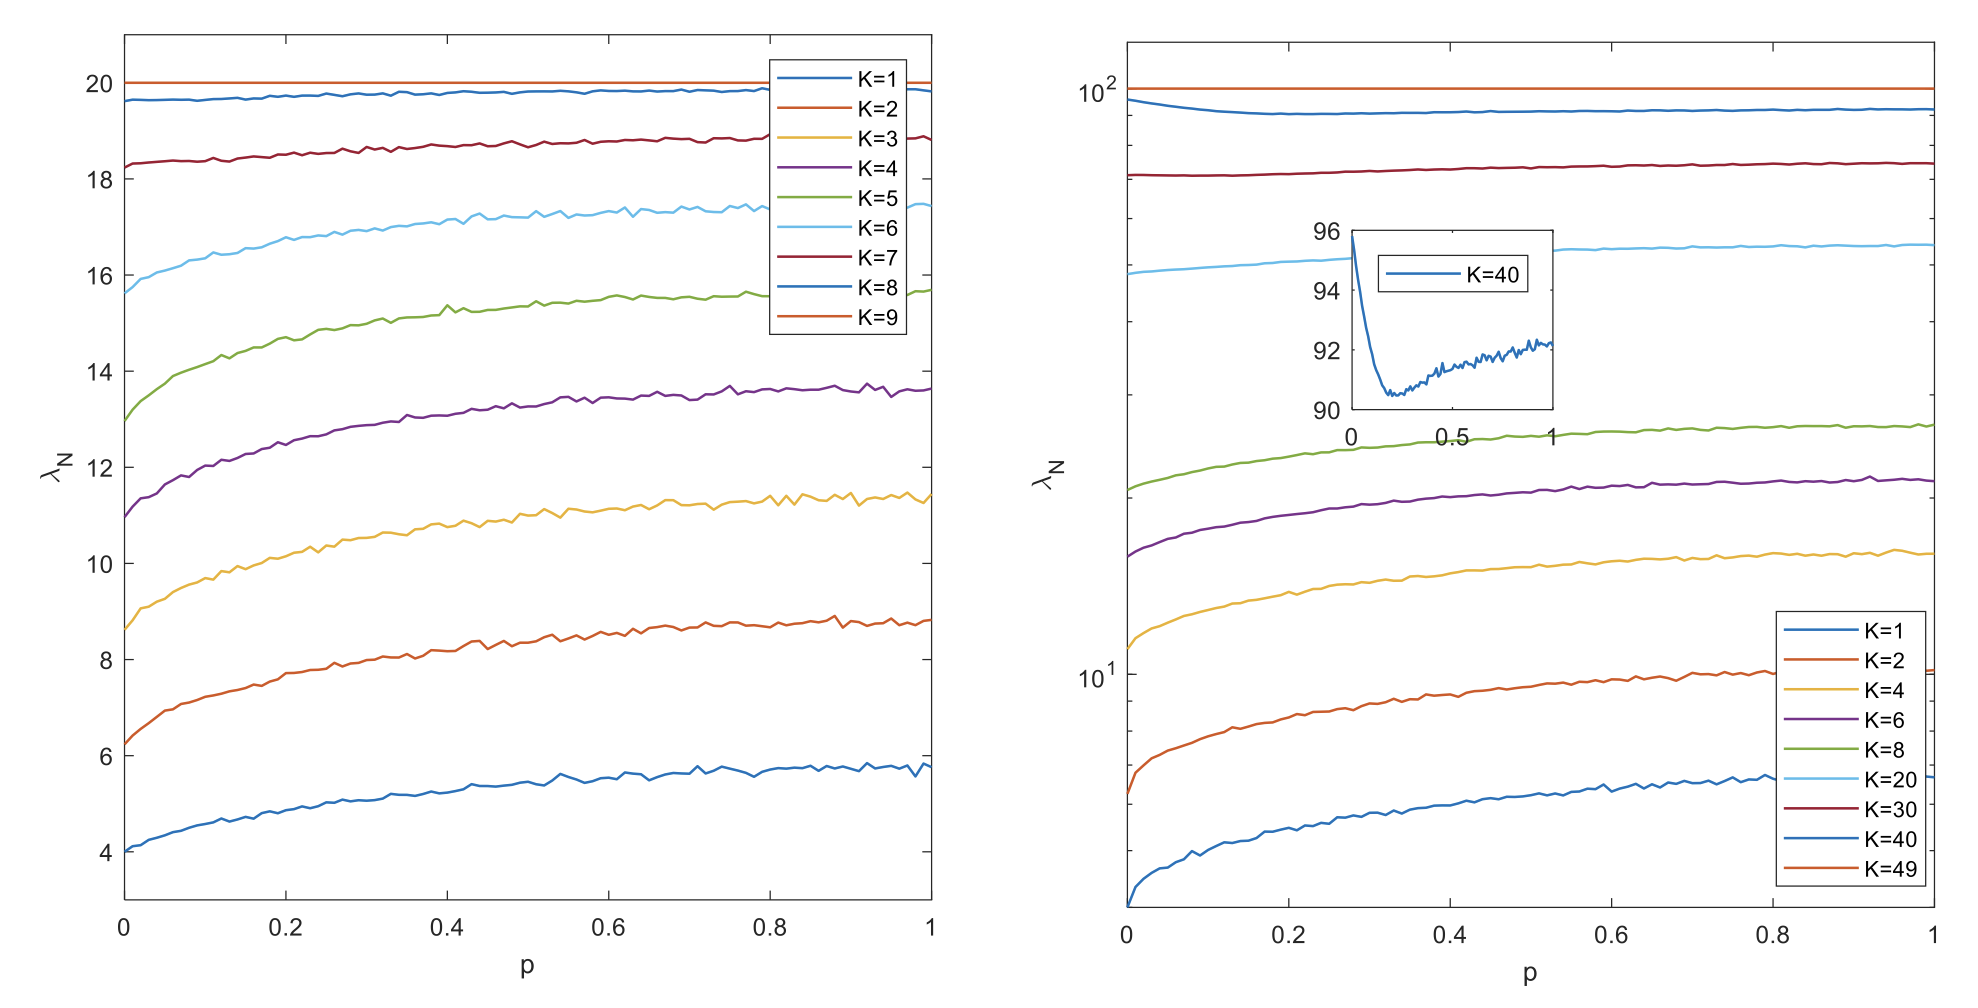
\includegraphics[width=\textwidth]{tb3.png}
\end{figure}
\section{小结} 